\documentclass[11pt]{article}
\usepackage{geometry, titlesec}
\usepackage[parfill]{parskip}
\usepackage[italicdiff]{physics}
\usepackage{amsfonts, amsthm}
\usepackage[cm]{fullpage}
\usepackage{fancyhdr}
\usepackage{enumitem}
\usepackage{xcolor, soul}
\usepackage{graphicx}
\usepackage[export]{adjustbox}
\usepackage{siunitx}
%\allowdisplaybreaks

\renewcommand{\thesubsection}{\thesection.\alph{subsection}}
\setenumerate[1]{label={(\alph*)}}

\makeatletter
\renewcommand*\env@cases[1][1.2]{%
  \let\@ifnextchar\new@ifnextchar
  \left\lbrace
  \def\arraystretch{#1}%
  \array{@{}l@{\quad}l@{}}%
}
\makeatother
 
\renewcommand{\footrulewidth}{.2pt}
%\setlist[enumerate]{leftmargin=*}
\pagestyle{fancy}
\fancyhf{}
\lhead{Physics 132-B}
\chead{\textbf{Discussion 3 Solutions}}
\rhead{A--De Discussion}
\setlength{\headheight}{11pt}
\setlength{\headsep}{11pt}
\setlength{\footskip}{24pt}
\lfoot{\today}
\rfoot{\thepage}

\titleformat{\subsection}[runin]{\normalfont\large\bfseries}{\thesubsection}{1em}{}
\newcommand{\refeq}[1]{(\ref{#1})}

\newcommand{\beq}{\begin{equation*}}
\newcommand{\eeq}{\end{equation*}}

\newcommand{\beqn}{\begin{equation}}
\newcommand{\eeqn}{\end{equation}}

\newcommand{\blg}{\begin{align*}}
\newcommand{\elg}{\end{align*}}


\newenvironment{statement}
{
    \color{gray}
    \ignorespaces
}
{
%    \smallskip
}

\newenvironment{problem}
{
    \color{darkgray}
    \ignorespaces
}

\newenvironment{solution}
{
    \color{black}
    \paragraph{Solution.}
    \ignorespaces
}
{
    \bigskip
}

\renewcommand{\vec}[1]{\mathbf{#1}}
\newcommand{\imgscale}{1.7}

\addtolength{\tabcolsep}{.2in}

\begin{document}
	

\newcommand{\vE}{\vec{E}}
\newcommand{\vF}{\vec{F}}

\paragraph{Question 23.1}
\begin{problem}
	A student asked, ``Since electrical potential is always proportional to potential energy, why bother with the concept of potential at all?''  How would you respond?
\end{problem}

\vfill

\newcommand{\vl}{\vec{l}}

\begin{minipage}{0.75\textwidth}
\paragraph{Question 23.9}
\begin{problem}
	If you carry out the integral of the electric field $\int \vE \cdot d\vl$ for a \emph{closed} path like that shown in Fig.~Q23.9, the integral will \emph{always} be equal to zero, independent of the shape of the path and independent of where charges may be located relative to the path.  Explain why.
\end{problem}
\end{minipage}%
\hspace{0.05\textwidth}%
\begin{minipage}{0.2\textwidth}
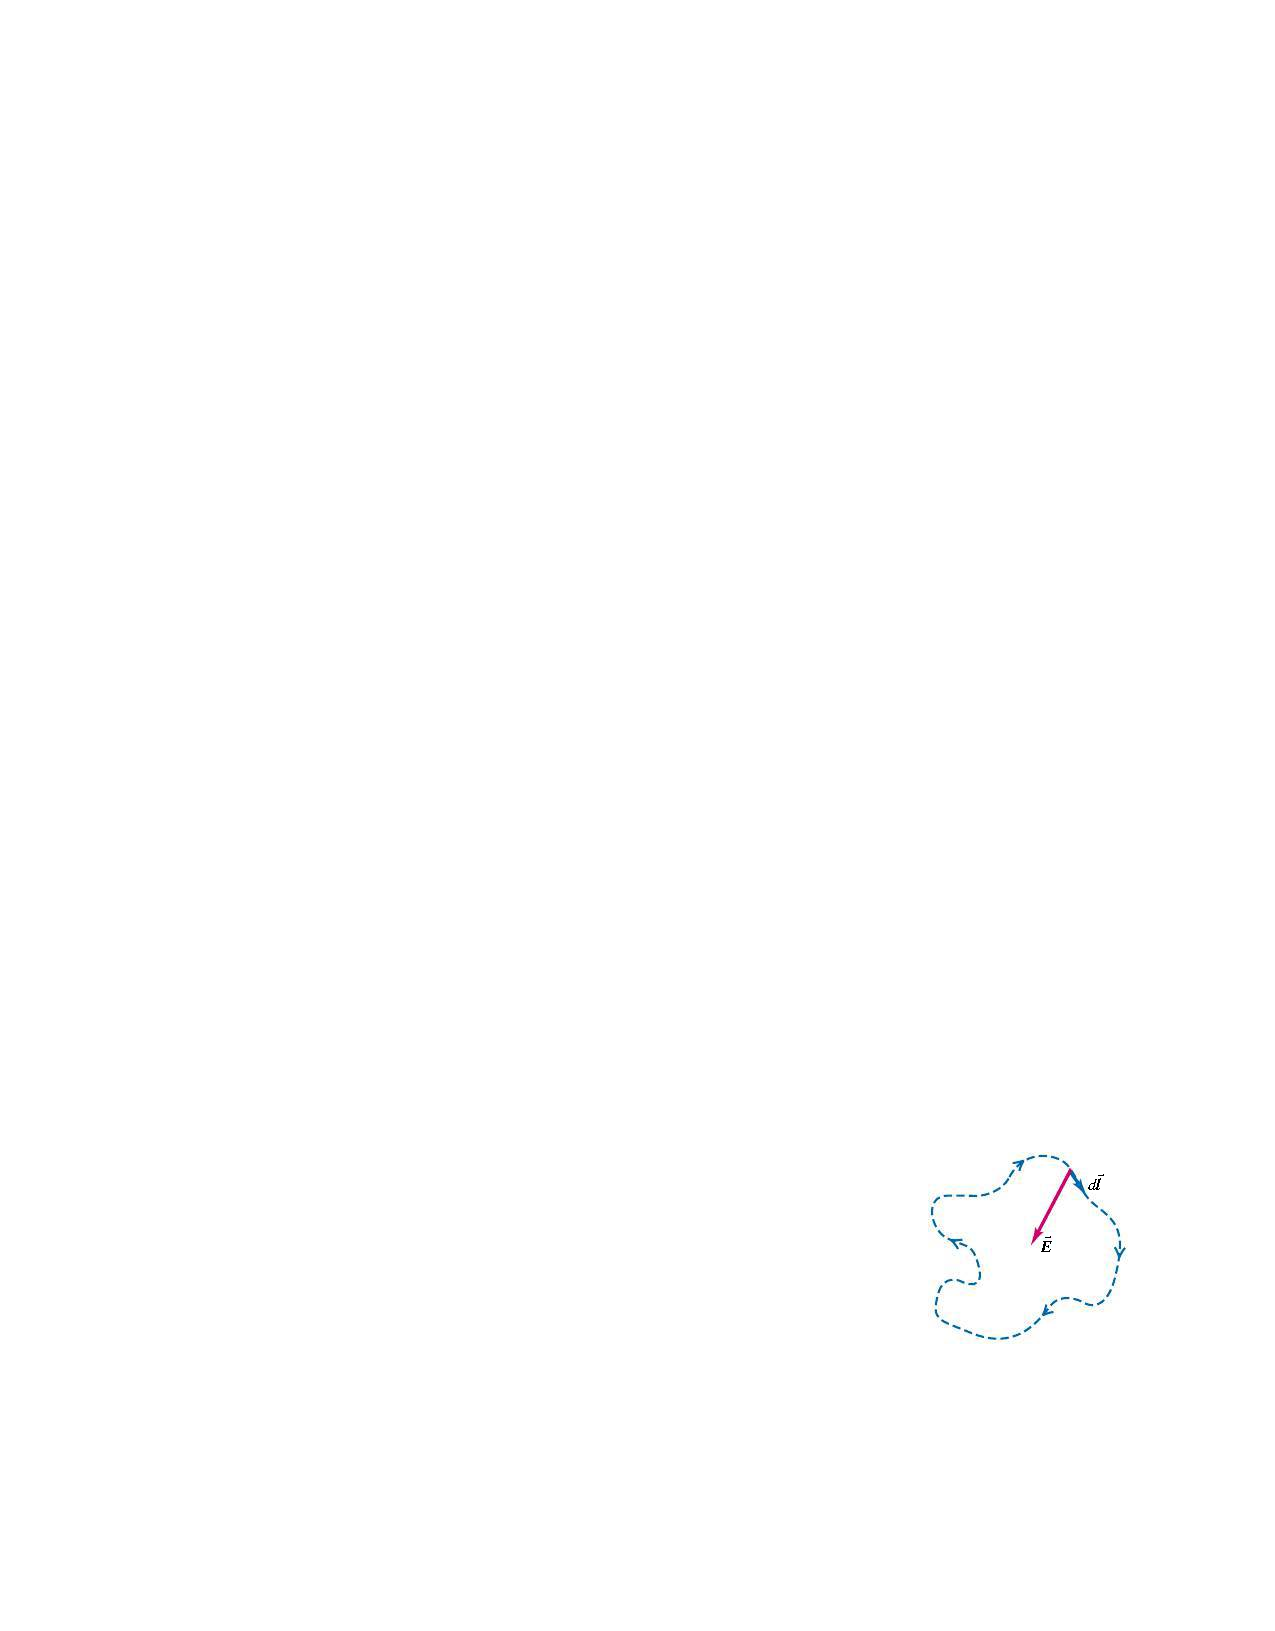
\includegraphics[center]{Q23-9}
\center \textbf{Fig.~Q23.9}
\end{minipage}

\begin{solution}
	This is related to a familiar concept from last quarter---work.  Just as $\Delta W = \int \vF \cdot d\vl$, $\Delta V = \int \vE \cdot d\vl$.  One of the very important things we learned about work is that it is path independent, meaning that the value of $W$ depends only on the endpoints and not how we travel between them.  This has special consequences for a closed loop: if we pick an object up off the floor and put it back down, we have done zero work.  Likewise, if we start at one point in space and return to it, the potential difference between our starting point and our ending point is obviously zero.
\end{solution}

\vfill

\begin{minipage}{0.6\textwidth}
\paragraph{Question 23.22}
\begin{problem}
	A positive point charge is placed near a very large conducting plane.  A professor of physics asserted that the field caused by this configuration would be the same as would be obtained by removing the plane and placing a negative point charge of equal magnitude in the mirror-image position behind the initial position of the plane.  Is this correct?  Why or why not?  (\emph{Hint:} Inspect Fig.~23.23b.)
\end{problem}
\end{minipage}%
\hspace{0.05\textwidth}%
\begin{minipage}{0.35\textwidth}
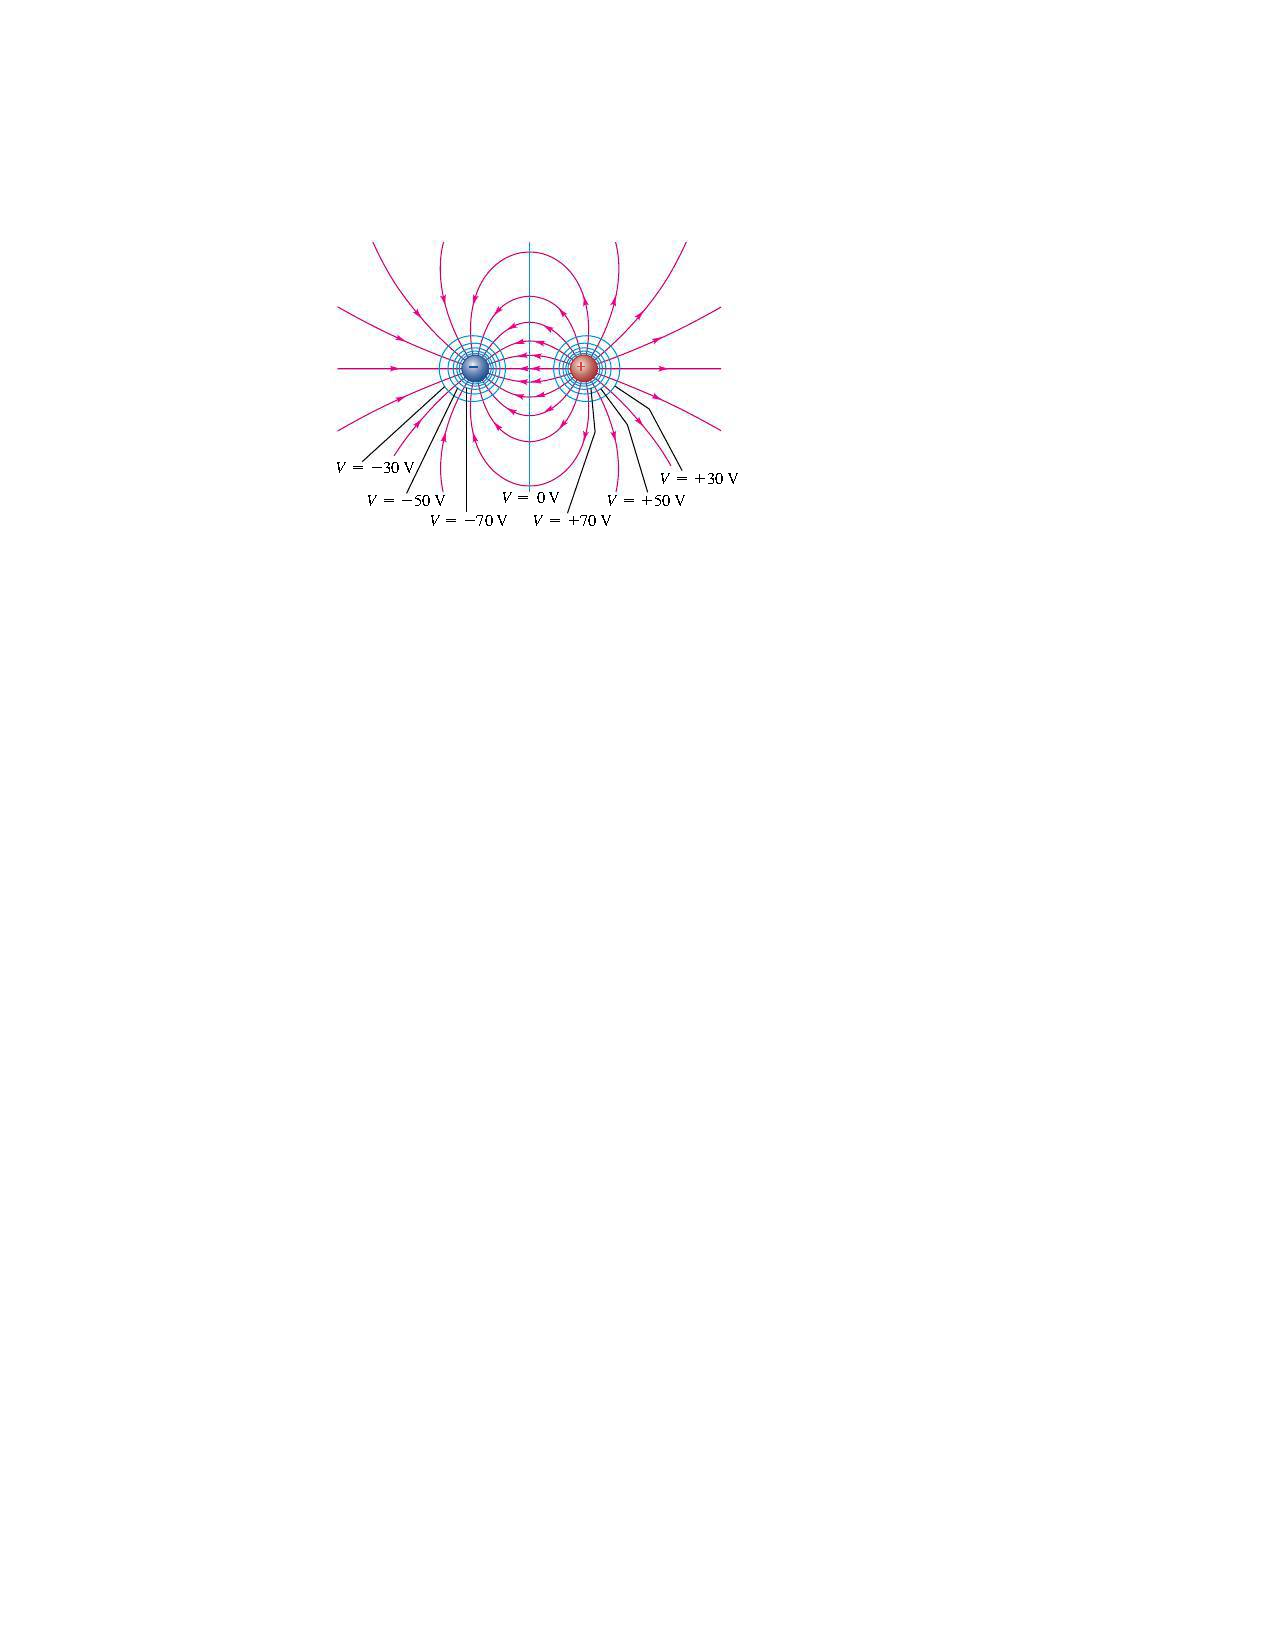
\includegraphics[center]{23-23b}
\center \textbf{Fig.~23.23b}
\end{minipage}

\begin{solution}
	This is related to a calculation technique called the method of images.  This method can be used to avoid doing the more difficult calculations that come along with charge distributions as opposed to point charges, which are comparatively easy to work with.  Imagine that, instead of the negative point charge $-q$ in the figure, we had a negatively charged plane of total charge $-q$ going down the middle.  The electric field lines on the right half of the figure would look exactly the same: they would come out radially from the positive point charge and end all along the conducting plane.  Of course, the electric field on the left half of the image would not be the same.
\end{solution}



\newcommand{\eo}{\epsilon_0}
\newcommand{\Vf}{V_f}
\newcommand{\Qf}{Q_f}
\newcommand{\Qi}{Q_i}

\paragraph{Problem 23.81}
\begin{problem}
	A heart cell can be modeled as a cylindrical shell that is \SI{100}{\micro\meter} long, with an outer diameter of \SI{20.0}{\micro\meter} and a cell wall thickness of \SI{1.00}{\micro\meter}.  Potassium ions move across the cell wall, depositing positive charge on the outer surface and leaving a net negative charge on the inner surface.  During the so-called resting phase, the inside of the cell has a potential that is \SI{90.0}{\milli\volt} lower than the potential on the outer surface.
	\begin{enumerate}
	
		\item If the net charge of the cell is zero, what is the magnitude of the total charge on either cell wall membrane?  Ignore edge effects and treat the cell as a very long cylinder.
		
		\begin{solution}
			We are told that we can treat the cell as a very log cylinder, which is a hint that we should work with the charge on the outer cell wall.  Just as the electric field outside a charged sphere is the same as for a point charge at its center, the electric field outside an infinitely long cylinder is the same as for a line charge along its axis.  We know from class that the electric field of an infinite line of charge is
			\beq
				\vE = \frac{1}{2\pi \eo} \frac{\lambda}{r} \,\vec{\hat{r}},
			\eeq
			where $\lambda$ is the linear charge density.  The total charge of the line, $Q$, is then related by $\lambda = Q / L$, where $L$ is the length of the line.  Here, $Q$ is the magnitude of the total charge on the outer cell wall.
			
			  We can now use $\vE$ to ?ind an expression for the potential difference $\Delta V$ across the cell wall.  The expression we found for $\vE$ is really only valid outside of the cell, but since the wall thickness is so small compared to the (effectively infinite) length of the cell, it should be okay for the purposes of our approximation to assume it is valid on the inner wall as well.
			  
			  We can integrate from the inner radius $a$ to the outer radius $b$, and solve for $Q$:
			\beq
				\Delta V = \int_a^b \vE \cdot d\vl
				= \int_a^b \frac{1}{2\pi \eo} \frac{\lambda}{r} \dd{r}
				= \frac{Q / L}{2 \pi \eo} \int_a^b \frac{\dd{r}}{r}
				= \frac{Q / L}{2 \pi \eo} \bigg[ \ln(r) \bigg]_a^b
				= \frac{Q / L}{2 \pi \eo} \ln\!\left( \frac{b}{a} \right)
				\implies
				Q = \frac{2\pi\eo L}{\ln(b/a)} \Delta V.
			\eeq
			We know $L = \SI{100}{\micro\meter}$.  The outer diameter of the cell is \SI{20.0}{\micro\meter}, so its outer radius $b = \SI{10.0}{\micro\meter}$.  Since the cell is \SI{1.00}{\micro\meter} thick, its inner radius $a = \SI{9.0}{\micro\meter}$.  We are told that $\Delta V$ across the cell is \SI{90.0}{\milli\volt}, going from the inside to the outside.  Plugging in these numbers,
			\beq
				Q = \frac{2\pi (\SI{8.85e-12}{\square\coulomb\per\newton\per\square\meter}) (\SI{100e-6}{\meter})}{\ln[(\SI{10.0e-6}{\meter}) / (\SI{9.0e-6}{\meter})]} (\SI{90.0e-3}{\newton\meter\per\coulomb})
				= \SI{4.75e-15}{\coulomb}.
			\eeq
\end{solution}


		\item What is the magnitude of the electric field just inside the cell wall?
		
		\begin{solution}
			Since we decided the experession $\vE$ we wrote applies on the inner cell wall, we can easily plug in $r = a = \SI{9.0}{\micro\meter}$ and the value we obtained for $Q$:
			\beq
				E(a) = \frac{1}{2\pi \eo} \frac{Q / L}{a}
				= \frac{1}{2\pi (\SI{8.85e-12}{\square\coulomb\per\newton\per\square\meter})} \frac{\SI{4.75e-15}{\coulomb}}{(\SI{100e-6}{\meter}) (\SI{9.0e-6}{\meter})}
				= \SI{9.49e3}{\volt\per\meter}.
			\eeq
		\end{solution}
		
		\clearpage
		\item In a subsequent depolarization event, sodium ions move through channels in the cell wall, so that the inner membrane becomes positively charged.  At the end of this event, the inside of the cell has a potential that is \SI{20.0}{\milli\volt} higher than the potential outside the cell.  If we model this event by charge moving from the outer membrane to the inner membrane, what magnitude of charge moves across the cell wall during this event?
		
		\begin{solution}
			We can use our formulation from (a) once more to solve for the total charge \emph{after} the depolarization event, which we'll call $\Qf$.  Note that the inner surface is now positively charged instead of negatively charged, so we need to use a minus sign on the new potential difference: $\Delta \Vf = -\SI{20.0}{\milli\volt}$.  Then
			\begin{align*}
				\Qf &= \frac{2\pi\eo L}{\ln(b/a)} \Delta \Vf
				= \frac{2\pi (\SI{8.85e-12}{\square\coulomb\per\newton\per\square\meter}) (\SI{100e-6}{\meter})}{\ln[(\SI{10.0e-6}{\meter}) / (\SI{9.0e-6}{\meter})]} (-\SI{20.0e-3}{\newton\meter\per\coulomb}) \\
				&= \SI{-1.06e-15}{\coulomb}.
			\end{align*}
			The magnitude of charge that has moved is now $|\Delta Q| = |\Qf - \Qi|$, where $\Qi$ is what we found in (a):
			\beq
				|\Delta Q| = |\Qf - \Qi|
				= |\SI{-1.06e-15}{\coulomb} - \SI{4.75e-15}{\coulomb}|
				= \SI{5.81e-15}{\coulomb}.
			\eeq
		\end{solution}
		
		
		\item If this were done entirely by the motion of sodium ions, Na$^+$, how many ions have moved?
		
		\begin{solution}
			Each sodium ion has a net charge of $+e$, where $e$ is the magnitude of the electron charge.  We can solve for the number of ions, $N$, by
			\beq
				N = \frac{\Delta Q}{e}
				= \frac{\SI{5.81e-15}{\coulomb}}{\SI{1.60e-19}{\coulomb}}
				\approx 36,300.
			\eeq
		\end{solution}
		
	\end{enumerate}
\end{problem}


\clearpage
\paragraph{Question 23.1}

\begin{solution}
	The beauty of electric potential is that it relates to the electric field $\vE$, and not the Coulomb force $\vF = q \vE$.  (Remember that electric potential is to electric field as potential energy is to force: $\vE = -\nabla V$ and $\vF = -\nabla U$.)  The magnitude of the electric field at any point in space has nothing to do with the charge $q$ of a hypothetical object we might want to place there.  The magnitude of the Coulomb force on that object, however, \emph{does} depend on $q$.  Likewise, the electric potential does not depend on $q$, while the potential energy does.  So the electric potential is valuable because it's completely universal---it potential can be applied to any object of any charge, while any potential energy that we calculate is ``married'' to one particular charge.
\end{solution}



\end{document}